\begin{esercizio}
   A particle of mass $m$ is in a potential well given by
   \begin{equation*}
      V(x)=
      \begin{cases}
         +\infty & \text{for } x<0\\
         0 & \text{for } x<0<\frac{L}{2}\\
         V_0 & \text{for } \frac{L}{2}<x<L\\
         +\infty & \text{for } x>L\\
      \end{cases}
   \end{equation*}
   \begin{enumerate}[label=\alph*), leftmargin=0.6cm]
      \item Use perturbation theory to calculate the energy of the ground state $E_1^{(1)}$.
      \item For $m=1 \; \rm GeV$ and $L=2 \; \rm fm$ what is the value of $V_0$ to have $V_0=2E_1^{(1)}$?
      \item Under the condition in b), ($V_0 \ll E$), calculate the ground state energy with the WKB approximation.
      \item How the result in c) compares to the result in a)? (Explain)
   \end{enumerate}
\end{esercizio}
\begin{soluzione}
   Svolgiamo il punto a). Per prima cosa rappresentiamo il potenziale:

   \begin{figure}[H]
      \centering
      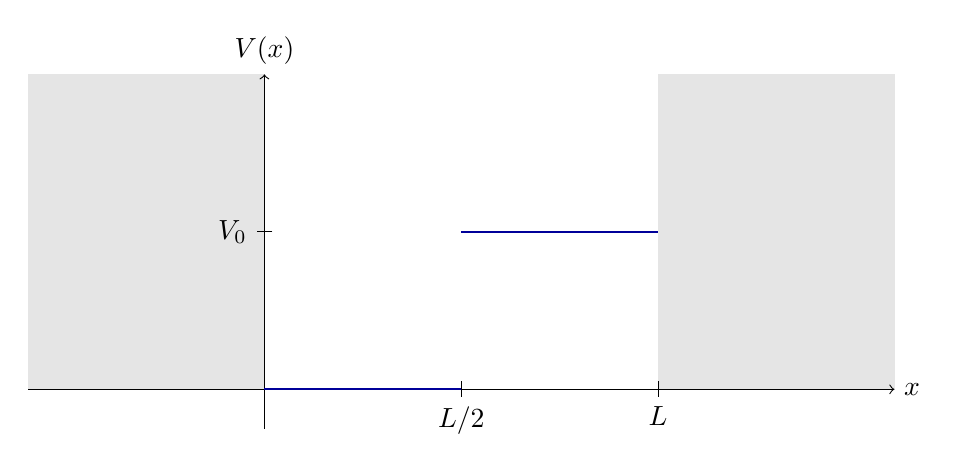
\begin{tikzpicture}
         \filldraw[gray!20!] (0,0) -- (0,4) -- (-3,4) -- (-3,0) -- cycle;
         \filldraw[gray!20!] (5,0) -- (5,4) -- (8,4) -- (8,0) -- cycle;
         \draw[->] (0,-0.5) -- (0,4) node[above] {$V(x)$};
         \draw[->] (-3,0) -- (8,0) node[right] {$x$};
         \draw[thick,blue!60!black] (0,0) -- (2.5,0);
         \draw[thick,blue!60!black] (2.5,2) -- (5,2);
         \draw (2.5,0.1) -- (2.5,-0.1) node[below] {$L/2$};
         \draw (5,0.1) -- (5,-0.1) node[below] {$L$};
         \draw (0.1,2) -- (-0.1,2) node[left] {$V_0$};
      \end{tikzpicture}
   \end{figure}

   Siamo ancora nell'ambito della teoria perturbativa, quindi dobbiamo identificare la correzione al potenziale imperturbato. Quest'ultimo è quello della buca quadra, dato da
   
   \begin{equation*}
      V_{\rm box}=
      \begin{cases}
         0 & \text{per } 0<x<L\\
         \infty & \text{altrimenti}\\
      \end{cases}
   \end{equation*}

   Le funzioni d'onda degli stati imperturbati sono date da
   
   \begin{equation*}
      \psi_n^{(0)}(x)
      =\sqrt{\frac{2}{L}} \sin{\qty( \frac{n \pi}{L} x)}
      \qq{,}
      n=1,2,\ldots
   \end{equation*}

   mentre le energie associate da

   \begin{equation*}
      E_n^{(0)}
      =\frac{\hbar^2 \pi^2 n^2}{2mL^2}
      \qq{,}
      n=1,2,\ldots
   \end{equation*}

   Riscriviamo quindi il potenziale $V$ come il potenziale $V_{\rm box}$ della buca quadra più un termine perturbativo $V'$. In particolare, quest'ultimo può essere scritto come
   
   \begin{equation*}
      \textstyle V'
      =V_0 \vartheta\qty(x - \frac{L}{2}) \vartheta (L - x)
   \end{equation*}
   
   dove le funzioni theta di Heaviside così fatte ci dicono che $V'$ contribuisce con un termine $V_0$ soltanto nella regione per $L/2<x<L$.
   
   A questo punto calcoliamo l'energia al primo ordine per il ground state. Per la teoria perturbativa indipendente dal tempo al primo ordine si ha che $E_1^{(1)}=E_1^{(0)} + \delta E_1^{(1)}$, dove la correzione al primo ordine $\delta E_1^{(1)}$ è data dall'elemento di matrice della perturbazione rispetto al ground state imperturbato del sistema:
   
   \begin{equation*}
      \delta E_1^{(1)}
      =\mel*{1^{(0)}}{V'(x)}{1^{(0)}}
      =\int_{-\infty}^{+\infty} \dd{x} \psi_1^*(x) V'(x) \psi_1(x)
   \end{equation*}

   Una volta che esplicitiamo $V(x)$, l'integrale risulta avere contributo non nullo soltanto nella regione per $L/2<x<L$, per cui
   \begin{equation*}
      \delta E_1^{(1)}
      =V_0 \int_{L/2}^{L} \dd{x} \frac{2}{L} \sin^2{ \qty( \frac{\pi x}{L} ) }
      =\frac{V_0}{L} \int_{L/2}^{L} \dd{x} \qty[ 1 - \cos{ \qty( \frac{2\pi x}{L} ) } ]
   \end{equation*}

   avendo usato la relazione trigonometrica $2 \sin^2{\alpha}=1 - \cos{(2\alpha)}$ nell'ultimo passaggio.

   Se adesso operiamo il cambiamento di variabile

   \begin{equation*}
      z=\frac{2\pi x}{L}
      \implies
      x=\frac{L z}{2\pi}
      \qq{,}
      \dd{x}=\frac{L \dd{z}}{2\pi}
   \end{equation*}

   Possiamo riscrivere l'integrale come

   \begin{equation*}
      \frac{V_0}{L} \int_{L/2}^{L} \dd{x} \qty[ 1 - \cos{ \qty( \frac{2\pi x}{L} ) } ]
      =\frac{V_0}{2\pi} \int_{\pi}^{2\pi} \dd{z} ( 1 - \cos{z} )
      =\frac{V_0}{2}
   \end{equation*}

   Abbiamo quindi trovato che la correzione al primo ordine al ground state imperturbato è pari a metà del potenziale. Il livello di energia corretto risulta dunque essere

   \begin{equation*}
      E_1^{(1)}
      =\frac{\hbar^2 \pi^2}{2mL^2} + \frac{V_0}{2}
   \end{equation*}
   
   Passiamo al punto b). Cerchiamo, fissati i valori forniti dal testo per la massa e per la larghezza della buca, il valore che deve avere $V_0$ per essere uguale a $0.2E_1^{(1)}$. Tale condizione può essere scritta come

   \begin{equation*}
      E_1^{(1)}=5V_0
      \iff
      \frac{\hbar^2 \pi^2}{2mL^2} + \frac{V_0}{2}=5V_0
      \implies
      V_0=\frac{\hbar^2 \pi^2}{9 m L^2}
   \end{equation*}

   Se in tale espressione estrapoliamo l'espressione dell'energia del ground state imperturbato possiamo scrivere ancora:

   \begin{equation*}
      V_0=\frac{\hbar^2 \pi^2}{9 m L^2}
      =\frac{2}{9} E_1^{(0)}
      \simeq 0.22 E_1^{(0)}
   \end{equation*}

   Da quest'ultima espressione deduciamo che $V_0 \sim 20\%E_1^{(0)}$ e che $\delta E_1^{(1)} \sim 10\%E_1^{(1)}$.

   A questo punto ricaviamo il valore di $V_0$ sostituendo i valori numerici. Cerchiamo di far spuntare quantità note moltiplicando e dividendo per $c^2$, in modo che al denominatore abbiamo la massa della particella che è data dal testo e al numeratore abbiamo la quantità $\hbar c$, che in questo caso conviene esprimere come $0.2 \; \rm GeV \, fm$:

   \begin{equation*}
      V_0
      =\frac{(\hbar c^2) \pi^2}{9 (mc^2) L^2}
      =\rm \frac{4 \cdot 10^{-2} \; GeV^2\,fm^2 \cdot 10}{9 \cdot 1 \; GeV \cdot 4 \; fm^2}
      =\frac{1}{90} \; GeV
      \approx 11 \; MeV
   \end{equation*}

   Passiamo ora al quesito c). Nella condizione $V_0 \ll E$ (in cui siamo perché $V_0 \sim 20\% E$, dobbiamo calcolare l'energia dello stato fondamentale con l'approssimazione WKB.
   
   In questo caso ci troviamo davanti ad una buca con due pareti verticali, quindi la condizione per ottenere i livelli di energie approssimati è
   
   \begin{equation*}
      \int_{x_1}^{x_2} p(x) \dd{x}=n\pi\hbar
      \qq{,}
      n=1,2,\ldots
   \end{equation*}

   Nel problema in esame i turning points $x_1$ e $x_2$ sono $x_1=0$ e $x_2=L$. Sostituendo poi l'espressione del potenziale otteniamo
   
   \begin{gather*}
      \int_{0}^{L} p(x) \dd{x}
      \int_{0}^{L} \sqrt{2m \bigl[ E - V(x) \bigr]} \dd{x}
      =\int_{0}^{L/2} \sqrt{2mE} \dd{x} + \int_{L/2}^{L} \sqrt{2m(E - V_0)} \dd{x}
      =\\
      =\sqrt{2mE} \frac{L}{2} + \sqrt{2m(E - V_0)} \frac{L}{2}
      =\sqrt{2m} \frac{L}{2} \qty( \sqrt{E} + \sqrt{E - V_0} )
      =n \pi \hbar
   \end{gather*}

   In particolare l'ultima uguaglianza può essere riscritta come

   \begin{equation*}
      \sqrt{E} + \sqrt{E - V_0}
      =\frac{2 n \pi \hbar}{\sqrt{2m} L}
   \end{equation*}

   A questo punto eleviamo entrambi i membri al quadrato:

   \begin{equation*}
      E + E - V_0 + 2\sqrt{E(E - V_0)}
      =\frac{4 n^2 \pi^2 \hbar^2}{2 m L^2}
      =4 E_n^{(0)}
   \end{equation*}

   A partire da tale relazione dobbiamo ricavare $E$. Per fare ciò isoliamo la radice al primo membro e poi eleviamo al quadrato:

   \begin{gather*}
      2\sqrt{E(E - V_0)}
      =4 E_n^{(0)} - 2E + V_0
      \\
      \implies
      4E(E - V_0)
      =16 \bigl( E_n^{(0)} \bigr)^2 + 4E^2 + V_0^2 - 16 E E_n^{(0)} - 4EV_0 + 8 V_0 E_n^{(0)}
      \\
      \implies
      16 \bigl( E_n^{(0)} \bigr)^2 + V_0^2 - 16 E E_n^{(0)} + 8 V_0 E_n^{(0)}=0
   \end{gather*}

   da cui infine si ottiene

   \begin{equation*}
      E=E_n^{(0)} + \frac{V_0}{2} + \frac{V_0^2}{16 E_n^{(0)}}
   \end{equation*}

   Notiamo che tale espressione è data dal risultato ottenuto con la teoria perturbativa più un termine aggiuntivo $\frac{V_0^2}{16 E_n^{(0)}}$. Se però adesso questo punto sfruttiamo la condizione $V_0 \ll E$ fornita dal testo, tale energia si riduce semplicemente a

   \begin{equation*}
      E_n^{(0)} + \frac{V_0}{2}
   \end{equation*}

   Che è l'espressione che si ottiene con la teoria perturbativa.
   
   Svolgiamo infine il punto d). Facciamo un confronto utilizzando i valori numerici ottenuti prima. Riscriviamo l'espressione dei livelli energetici ottenuti per la WKB nel caso $n=1$ come
   
   \begin{equation*}
      E=E_1^{(0)} + \frac{V_0}{2} \qty( 1 + \frac{V_0}{8 E_1^{(0)}} )
   \end{equation*}

   Utilizzando i valori $V_0=1.1 \cdot 10^{-2} \; \rm GeV$, $E_1^{(0)}=5V_0=5 \cdot 10^{-2} \; \rm GeV$, si trova che $\frac{V_0}{8 E_1^{(0)}} \approx 0.03 \ll 1$. Possiamo allora effettivamente dire che, per i valori trovati nel punto b), siamo nel caso in cui tale termine risulta trascurabile e pertanto il risultato della WKB coincide con quello della teoria perturbativa.
\end{soluzione}

\newpage
\setcounter{equation}{0}

\begin{esercizio}
   An electron is in a potential given by
   \begin{equation*}
      V(x)=
      \begin{dcases}
         \infty & \text{for } x<0\\
         0 & \text{for } 0<x<\frac{L}{2}\\
         V_0 \qty( \frac{2x}{L} - 1 ) & \text{for } \frac{L}{2}<x<L\\
         \infty & \text{for } x>L\\
      \end{dcases}
   \end{equation*}
   \begin{enumerate}[label=\alph*), leftmargin=0.6cm]
      \item Use perturbation theory to calculate the energy\footnotemark\;of the ground state.
      \item What is the condition on $V_0$ to have perturbation theory valid?
      \item Put $V(x)=0$ for $x>L$ and $E<V_0$. Use WKB to calculate the penetrability of the barrier for $V_0=4 \; \rm MeV$, $L=10 \; \rm fm$ and $E=V_0/2$.
   \end{enumerate}
\end{esercizio}
\begin{soluzione}
   \footnotetext{Quando nel testo non è specificato, si intende fin al primo ordine.}

   Per prima cosa riportiamo in un grafico l'andamento del potenziale:

   \begin{figure}[H]
      \centering
      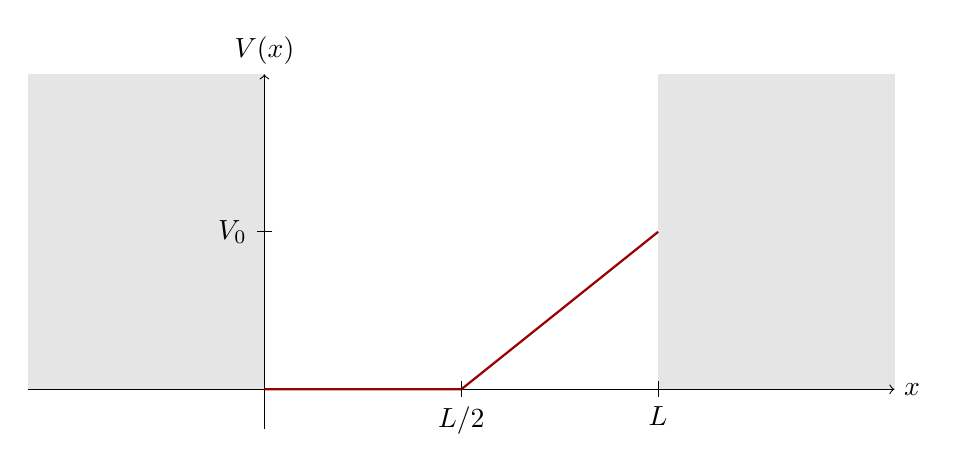
\begin{tikzpicture}
         \filldraw[gray!20!] (0,0) -- (0,4) -- (-3,4) -- (-3,0) -- cycle;
         \filldraw[gray!20!] (5,0) -- (5,4) -- (8,4) -- (8,0) -- cycle;
         \draw[->] (0,-0.5) -- (0,4) node[above] {$V(x)$};
         \draw[->] (-3,0) -- (8,0) node[right] {$x$};
         \draw[thick,red!60!black!] (0,0) -- (2.5,0) -- (5,2);
         \draw (2.5,0.1) -- (2.5,-0.1) node[below] {$L/2$};
         \draw (5,0.1) -- (5,-0.1) node[below] {$L$};
         \draw (0.1,2) -- (-0.1,2) node[left] {$V_0$};
      \end{tikzpicture}
   \end{figure}
   
   Svolgiamo il punto a). La correzione al primo ordine all'energia del ground state è data da
   
   \begin{gather*}
      \delta E_1^{(1)}
      =\mel*{\psi_1^{(0)}}{V'}{\psi_1^{(0)}}
      =\int_{L/2}^{L} \dd{x} V_0 \qty( \frac{2x}{L} - 1 ) \bigl| \psi_1^{(0)} \bigr|^2
      =\int_{L/2}^{L} \dd{x} V_0 \qty( \frac{2x}{L} - 1 ) \frac{2}{L} \sin^2{ \qty( \frac{\pi x}{L} ) }=
      \\
      =\frac{V_0}{L} \qty[ \int_{L/2}^{L} \dd{x} \qty( \frac{2x}{L} - 1 ) - \int_{L/2}^{L} \dd{x} \qty( \frac{2x}{L} - 1 ) \cos{\qty( \frac{2\pi x}{L} )}]
   \end{gather*}
   dove abbiamo sfruttato la relazione trigonometrica $2 \sin^2{\alpha}=1 - \cos{(2\alpha)}$ nell'ultimo passaggio.

   Calcoliamo adesso ciascun integrale: per il primo si ha banalmente

   \begin{equation*}
      \int_{L/2}^{L} \dd{x} \qty( \frac{2x}{L} - 1 )
      =\qty[ \frac{x^2}{L} - x]_{L/2}^{L}
      =L - L - \frac{L}{4} + \frac{L}{2}
      =\frac{L}{4}
   \end{equation*}

   Per quanto riguarda il secondo integrale, esso si può ulteriormente spezzare in due integrali:

   \begin{equation*}
      \int_{L/2}^{L} \dd{x} \qty( \frac{2x}{L} - 1 ) \cos{\qty( \frac{2\pi x}{L} )}
      =\int_{L/2}^{L} \dd{x} \frac{2x}{L} \cos{\qty( \frac{2\pi x}{L} )} - \int_{L/2}^{L} \dd{x} \cos{\qty( \frac{2\pi x}{L} )}
   \end{equation*}

   i quali, ponendo

   \begin{equation*}
      y=\frac{2\pi x}{L}
      \implies
      \dd{y}=\frac{2\pi \dd{x}}{L}
   \end{equation*}

   Possono esse riscritti come

   \begin{equation*}
      \frac{L}{2\pi^2} \int_{\pi}^{2\pi} \dd{y} y \cos{y} - \frac{L}{2\pi} \int_{\pi}^{2\pi} \dd{y} \cos{y}
   \end{equation*}

   Per il secondo integrale otteniamo subito che
   
   \begin{equation*}
      \frac{L}{2\pi} \int_{\pi}^{2\pi} \dd{y} \cos{y}
      =\frac{L}{2\pi} \qty[ \sin{y} ]_{\pi}^{2\pi}
      =0
   \end{equation*}

   Il primo invece va risolto per parti: ponendo $f=y$ e $g=\cos{y}$, si ha

   \begin{equation*}
      \frac{L}{2\pi^2} \int_{\pi}^{2\pi} y \cos{y} \dd{y}
      =\frac{L}{2\pi^2} \qty{ \bigl[ y \sin{y} \bigr]_{\pi}^{2\pi} - \int_{\pi}^{2\pi} \sin{y} \dd{y} }
      =\frac{L}{2\pi^2} \bigl[ \cos{y} \bigr]_{\pi}^{2\pi}
      =\frac{L}{\pi^2}
   \end{equation*}

   Mettendo insieme i vari contributi troviamo che

   \begin{equation*}
      \delta E_1^{(1)}
      =\frac{V_0}{L} \qty( \frac{L}{4} - \frac{L}{\pi^2} )
      =V_0\qty( \frac{1}{4} - \frac{1}{\pi^2} )
   \end{equation*}

   e pertanto l'energia del ground state corretta al primo ordine risulta essere

   \begin{equation*}
      E_1^{(1)}
      E_1^{(0)} + \delta E_1^{(1)}
      =\frac{\pi \hbar^2}{m L^2} + V_0\qty( \frac{1}{4} - \frac{1}{\pi^2} )
   \end{equation*}

   Passiamo al punto b). Ricordiamo che la condizione affinché la teoria perturbativa sia valida è che il rapporto tra la correzione di energia e la differenza di energia tra lo stato imperturbato e quello più vicino deve essere molto minore di 1; in particolare per il ground state si deve avere
   
   \begin{equation*}
      \qty| \frac{\delta E_1^{(1)}}{E_1^{(0)} - E_2^{(0)}} | \ll 1
   \end{equation*}

   Esplicitando quanto trovato, tale condizione si riscrive come

   \begin{equation*}
      \qty| \frac{V_0\qty( \frac{1}{4} - \frac{1}{\pi^2} )}{-3 \frac{\hbar^2 \pi^2}{2 m L^2}} |
      =\frac{mL^2 V_0 (\pi^2 - 4)}{6\hbar^2}
      \ll 1
   \end{equation*}

   da cui si ricava che la condizione per $V_0$ è

   \begin{equation*}
      V_0 \ll \frac{6\hbar^2}{m L^2 (\pi^2 - 4)}
   \end{equation*}
   
   Svolgiamo ora il punto c). Adesso il potenziale cambia e diventa nullo nella regione per $xL$, dunque graficamente adesso la situazione è la seguente:
   
   \begin{figure}[H]
      \centering
      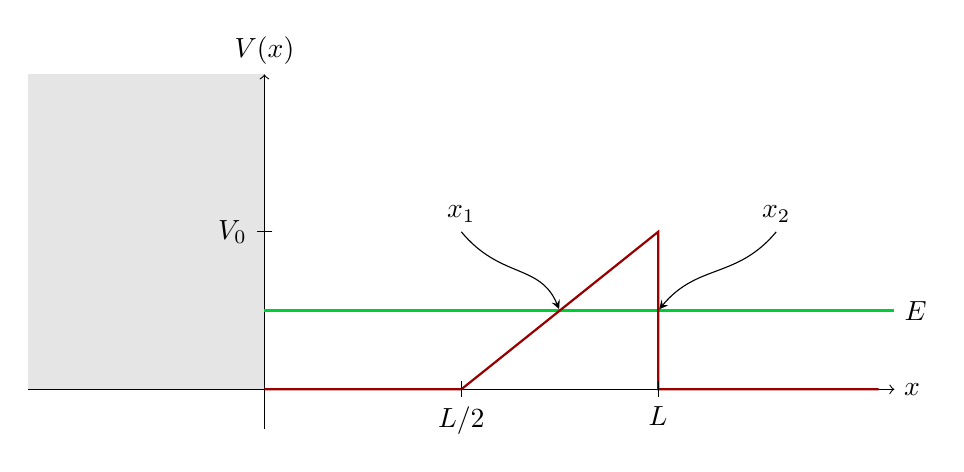
\begin{tikzpicture}
         \filldraw[gray!20!] (0,0) -- (0,4) -- (-3,4) -- (-3,0) -- cycle;
         \draw[->] (0,-0.5) -- (0,4) node[above] {$V(x)$};
         \draw[->] (-3,0) -- (8,0) node[right] {$x$};
         \draw[thick,green!60!teal!] (0,1) -- (8,1) node[right,black] {$E$};
         \draw[thick,red!60!black!] (0,0) -- (2.5,0) -- (5,2) -- (5,0) -- (7.8,0);
         \draw (2.5,0.1) -- (2.5,-0.1) node[below] {$L/2$};
         \draw (5,0.1) -- (5,-0.1) node[below] {$L$};
         \draw (0.1,2) -- (-0.1,2) node[left] {$V_0$};
         \draw[-stealth,shorten >= 0.6pt] (6.5,2) node[above] {$x_2$} .. controls (6,1.4) and (5.5,1.6) .. (5,1);
         \draw[-stealth,shorten >= 0.6pt] (2.5,2) node[above] {$x_1$} .. controls (3,1.4) and (3.5,1.6) .. (3.75,1);
      \end{tikzpicture}
   \end{figure}

   In questo caso dobbiamo usare la WKB per calcolare la penetrabilità della barriera (quindi siamo nel caso in cui $E<V_0$), che è data da

   \begin{equation*}
      T
      \approx \exp{ -\frac{2}{\hbar} \int_{x_1}^{x_2} \dd{x} \sqrt{ 2m \bigl[ V(x) - E \bigr] } }
   \end{equation*}

   dove $x_1$ e $x_2$ sono i turning points. La prima cosa da fare è proprio individuare questi ultimi. Si intuisce facilmente che $x_2=L$, mentre per $x_1$ dobbiamo uguagliare energia e potenziale:

   \begin{equation*}
      E=V_0\qty( \frac{2x_1}{L} - 1 )
      \implies
      x_1
      =\frac{L}{2}\qty( \frac{E}{V_0} + 1 )
   \end{equation*}

   Se adesso applichiamo la condizione fornita dal testo per cui $E=V_0/2$, troviamo che

   \begin{equation*}
      x_1
      =\frac{L}{2}\qty( \frac{V_0}{2V_0} + 1 )
      =\frac{3}{4} L
   \end{equation*}

   Possiamo quindi calcolare

   \begin{gather*}
      T
      =\exp{ -\frac{2}{\hbar} \int_{x_1}^{x_2} \dd{x} \sqrt{ 2m \qty[ V_0\qty( \frac{2x}{L} - 1 ) - E ] } }
   \end{gather*}

   Introduciamo la variabile

   \begin{equation*}
      z=2m \qty[ V_0\qty( \frac{2x}{L} - 1 ) - E ]
      \implies
      \dd{z}=\frac{4mV_0}{L} \dd{x}
   \end{equation*}

   da cui segue che

   \begin{gather*}
      z_1
      =2m \qty[ V_0\qty( \frac{2x_1}{L} - 1 ) - E ]
      =2m \qty{ V_0\qty[ \frac{2}{L} \frac{L}{2}\qty( \frac{E}{V_0} + 1 ) - 1 ] - E }
      =0
      \\[0.1cm]
      z_2
      =2m \qty[ V_0\qty( \frac{2x_2}{L} - 1 ) - E ]
      =2m (V_0 - E)
   \end{gather*}

   Usando tale cambio di variabile, l'integrale si può riscrivere come

   \begin{equation*}
      T
      \approx
      \exp{ -\frac{2L}{4 m V_0 \hbar} \int_{0}^{2m(V_0 - E)} \dd{z} \sqrt{z} }
      =\exp{ -\frac{L}{3 m \hbar V_0} \bigl[ 2m(V_0 - E) \bigr]^{\frac{3}{2}} }
   \end{equation*}

   Passiamo infine il punto d). Per prima cosa moltiplichiamo e dividiamo per $c^3$ in modo da far spuntare quantità note, in particolare $\hbar c$ e $mc^2$. Sostituendo poi i valori numerici forniti dal testo, si ha

   \begin{gather*}
      T
      \approx \exp{ - \frac{L}{3 mc^2 \hbar c V_0} \bigl[ 2 mc^2 (V_0 - E) \bigr]^{\frac{3}{2}} }
      =\\
      =\rm \exp{ - \frac{10 \; fm}{0.5 \; MeV \cdot 2 \cdot 10^2 \; MeV \, fm \cdot 3 \cdot 4 \; MeV} \bigl[ 2 \cdot 0.5 \; MeV (4 - 2) MeV \bigr]^{\frac{3}{2}} }
      =\\
      =\exp{ -\frac{1}{120} 2^{\frac{3}{2}} }
      =\exp{-\frac{\sqrt{2}}{60}}
      =0.98
   \end{gather*}
\end{soluzione}

\comment{

\newpage
\setcounter{equation}{0}

\begin{esercizio}
   A bi-atomic molecule is composed by two identical nuclei. The potential of the system is
   \begin{equation}
      U_{\rm tot}=U\qty( \qty| \vb{r} + \frac{\vb{a}}{2} | ) + U\qty( \qty| \vb{r} - \frac{\vb{a}}{2} | )
   \end{equation}
   The two nuclei have the centres at a distance $|\vb{a}|$ and $U(|\vb{r}|)=0$. $0<r<r_0$ and 0 elsewhere.
   \begin{enumerate}[label=\alph*), leftmargin=0.6cm]
      \item Calculate the differential cross section in first order Born approximation for a particle of mass $m$ in terms of the exchanged momentum $\vb{q}$.
      \item What is the differential cross section in the limit $|\vb{q}| \ll |\vb{a}|^{-1}$.
   \end{enumerate}
\end{esercizio}
\begin{soluzione}
   Poi stessa, prima che è è io non avevo capito una cosa, cioè il discorso di inserire c per ottenere la massa In questo caso, sì, funziona perché funziona, però come dovrei raggiungere se vedo cose in genere? No, se mi posta anche io quando ho fatto al vizio, mi sono chiesto chiesto deve funzionare Cioè, più che altro mi è venuto a piangere quando ho visto mh tagliato sotto, ho detto come faccio Allora, io ho c4 qua e io metto i c4 Ok, al cubo E il c cubo sotto, quindi ho metto un c cubo sotto, come ho messo? E ho metto un c cubo sopra Ora, se questo c cubo lo metto qua dentro Dientaci alla sess... no, ho detto la lavorata C4, certo Poi posso fare il contro certo, c4 elevato a 3 mezzi di venta c cubo Certo, perché l'ho elevato a 2 di viso 3 Quindi diciamo se volo di fioltare, perché io capisco che a me me ho fatto le uocemente a volte le queste parti le faccio Le uocemente è sul momento di basperare Quindi, quello che farei so che deve essere così, proprio faccio il controllo Sì, tutta più sé, se non riesco a farlo Ok, ok, grazie Altri tutti domande Sì, grazie Non lo credo mai, che se ne dico solo un po' di bionto Che cosa? Sotto al controllo del bionto Quelle bionto dentro, uno tranquillo di bionto C'è un uocello che si tratta tratta una cosa C'è un uocello che che che che che che che che che che che che che che che
   
   C'è un un un un un un una una una un uocello uocello uocello uocello uocello una cosa cosa cosa cosa cosa cosa cosa cosa una una C'è un un un un un un un un un un un un un un un un un C'è un uocello che si tratta di di cosa C'è un uocello uocello uocello tratta tratta tratta tratta tratta tratta uocello che che che che che che C'è C'è C'è C'è C'è C'è C'è C'è C'è Allora, vabbè, la sua copaccia e la la la le sue sue sue sue sue sue sue le sue sue sue l'idea è che ne studiamo il caso in cui c'è una regione e lo spazio è un certo potenziale di quindi ha un certo range del potenziale e vogliamo abbiamo un nome incidente e cosa succederà? Quali sarà la società? Che cosa doserà? Un'onda uscente più un'onda sfegha che che è una uscente più un'onda sfegha unile Il risultato sarà se lo avete spesso così questo è un regolo per parte della notazione che è un un più sottuale questa questa è un'onda uscente che è uscente questa è un'onda sfegha però è che è una sfegha a quella che poi è proprio l'obiettivo della teoria dello scattering che dobbiamo determinare la piezza di scattering quindi l'obiettivo è determinare questa piezza di scattering per cui possiamo tenere la sezione del punto di differential di queste che le chiamiamo in un punto di scattering e poi da questa che è un ruotore la sezione del punto di differential e a sin il 3 e a omega per qua la modulo 4 di questa piezza di scattering e vabbè chiaramente se vuoi ottenere la sezione tutto d'ultronde il punto di granere dell'angolo solido e ci sono in genere due metodi per andare in conto e risolvere il più bello scattering non è quello della partial wave analysis che però di non faremo e l'altro è quello della prossima azione di borg quindi ora faremo un esercizio della prossima azione di borg e nel caso della prossima azione di borg quello che si trova al primo ordine sempre che però alla fine è sempre il mio e che consideriamo è che la sezione tutto di borg in termini è chiaramente l'1k1 che prima si riferisce genres genres per quello che ha ha i k-tri e con i secoli questo è il il a meno 1 con 4 i d e co 2 e a 3 al 4 integrale 1 e 3 x e vado a i k-m e k-trimo x che è il potenziale x. Ora quello che si fa spesso esprimere in termini del momento transfer, del momento trasferito e quindi questa diventa, in primo qui, meno m2, che si trie con un attentato quadro integrale dentro x, di e elevato a iq, da questo momento l'asferito, x di i. Quindi q per come definito qui è k, k a meno k prima. In anche il libido potreste trovare al contrario, cioè definito come al finale nell'iniziale, in stel caso ci sarebbe il meno davanti. Usate la formula di controllare quale è q. Questa è il momento trasferito. Ci sono dei casi in cui questa formula che già alla termina, ovviamente ovviamente formula, cosa ci dice? C'è che l'ampiazza di scattering è la trasformata di furia e l'errore del potenziale, quindi è facile da ricordare a parte del fattore. Però ci sono casi in cui si semplificano terrumente nel caso di potenziale centrale, ovvero potenziale a simmetria sferica, ma vedremo che si applica in realtà a parte che non c'è la simmetria a 5 minuti. In questo caso è il formato di k, dove k cos'è l'angolo, la k è k prima. Quindi questo è k prima, questo è k prima, quindi è è è è è questa volta lo trovate espresso mettendo l'R qui, q r in modo che hai a vedere a porto 0 x y, quindi qua c'è un R qua. Quindi fate sempre attenzione a non sbagliare con gli esponenti. Quindi q, una altra cosa in formazione che è molto sempre è che si può vedere, diciamo che è un ruolo fuori da un'espressione, così questo è il del fattore. Si può vedere che il modulo di questo momento è la trasfer, è uguale a 2k per seno di data mezzi. Il modulo sono quali in un q z. Poi questo ci dovete dovete con qualche esercizio in questo totimo allo dei maxi, trovare i bimbi, quindi quindi vedete necessità di tevalo durante un compito. E di atomica molècule è composto di R più a mezzi più u di R meno mezzi e il modulo di Q di R R a a a a a R più a a a a a a a a a a uguale a meno di 0 per R tra 0 ed R con 0 e n0 è suo. E' una una di di di una traccia di calcolazione di di di di calcolazione di un q z.

   non è così non è è è per un po' di suentare in un'elettizia in genere c'è un aiuto che di capo c'è dice di valutare prima dei scattri in campi tutte per questo potenziale qui che è appunto per R da 0 e R0 e poi far un cambio di variabile integrazione per calcolare quello richiesto dal problema questo qua potenziale così penso che l'ho già trattato un esempio per solità il greco sono sbaglio però posso anche se lo faccio a wave questo è un momento di ricorda vabbè potrebbe fare questo che vi domande io comunque ma che la faccio con esempio veloce quindi questo qua ci porto a trovare trovare esercizi semplicemente con questo potenziale in questo caso abbiamo 2 nuclei, ognuno dei quali ha potenziale genere quindi ogni nuve, quindi abbiamo una molecola che ovviamente sono i 2 nuclei questa distanza è 2a o a e a e ognuno di queste ha un potenziale che approssimiamo con un potenziale costante entro un range che è quello quello questo raggio che considero R con 0 quindi ha prasciuzione di borne quindi possiamo iniziare a scrivere la forma che vedete prima F borne di K di K è K primo e a a m2 di greco è parolato 4 integrale in T3 il signo e alla meno il Q primo ma vedete il più molto grande dividete il conizio dove questo B è appunto la somma dei 2 potenziali però così mi sarebbe complicato se ricordi insieme quindi considero separatamente ciascuno dei 2 integrali quindi con ciascun termine separatamente e quindi consideriamo il primo quello con questo qua quindi in questo caso io andrei a guardare integrale di T3 il Q primo dire meno il Q il Q primo per U, P, R, Q, a mezzo per cui sarà in meno l'esperienza ah perché poi l'ho definita al contrario questo è quel discorso che dicevo prima allora io l'ho fatto tutto col meno quindi sotto possibilito ora facciamo col meno così sei con un leco scritto e poi con le lecchie oppure lo facciamo insieme in corretto però poi lo sto attendo perché ho troppo di esperienza allora rimaniamo con le lecchie quindi quando è espresso perché poi mi divenne da libre e mi base a quando l'ho fatto ovviamente quindi in questo caso è finale meno iniziamo giusto? questo è è sì, questo è il primo iniziamo, iniziamo inizia inizia meno finale quanto è possibile questo è il finale perfetto quindi dobbiamo risolvere questo che siamo nel caso a sigla di sferica quindi central potential quindi quello che dobbiamo andare a risolvere è del 3R è meno I Q, R Q, R Q, mezzi ora facciamo un cambio di variabili in cui mettiamo z, il quale R, che lo metti così che ci metti in questa situazione qua in diventa integrale in dentro di z è meno I z z sì è più I Q mezzi Q z e ora faccio un altro massaggio per il modo di avere qualcosa che sia veramente come cioè ora come potremmo farlo diciamo iniziava questo passaggio però per non comprendere mi l'ho fatto in tutto così, sto parendo una x uguale a z, a modo di z, ok? Il modo da vedere è proprio fatto che sia spericamente semplice. Allora questo risulta a e, e2 a mezzi, quindi ho tirato fuori questo termine, integrale da zero al finito, di tx, di x4, a fu con x, e poi ho il termine col t cosenteta, e questo qua è quello che quando l'intermettiamo abbiamo scritto prima nel caso di potenziale centrale. Quindi risulta e c'è il pi grego del delta phi che metto qua, integrale del phi lo tiro fuori, non d'angolo tentale. E in questo risulta su quale a 4 di grego q è elevato a e2 a mezzi integrale da zero al finito, e xx2 con x, zero di q con x. Ora io so che u x è divesso da zero solo per x tra zero e re con zero, e in questo caso è precedentemente uguale a meno di con zero. Quindi questo qua diventa meno di con zero, 4 di grego di viso q, e elevato a e2 pro scala le con mezzi integrale da zero a re con zero per la regione in cui non cui non e xx, e xx, e xx, E elevato a q, e elevato e elevato pu ametti, sento di q per re con zero meno q per re con zero coseno i pu per re con zero. Fondamente a parte il fattore e a parte questa esplorenziale che viene dal fatto che il centro della mollegola è esci stato di alfameggi rispetto al centro del nostro istituto di perimento di prendermo, abbiamo il risultato che troverete anche in molti di questi perveri in altri esercizi, principalmente di un potenziale, quello che diciamo in inizio, un potenziale uguale a meno di con zero. In questo caso abbiamo un suo fattore in più, e chiaramente se prendiamo l'altra parte, esplorati a passaggi anale, in cui con z, a delito, stavolta, a re, meno a fa mezzi, trovate la stessa identitiv cosa, ma qua abbiamo più o meno. Quindi lo scrivo, abbiamo che è l'integrale, indetre x, più, di e meno i pu, di x prima, di u, di r meno mezzi. E' uguale a meno quattro di tre campi con zero, di q e alla meno i pu a mezzi, se è uno di q con il recon zero, meno q e il recon zero, coseno di q e il recon zero. Facendo la somma dei due termi, ok, quindi parto da qui nella prima. All'interno, ho finito tutto chiaro. 
   
   Quindi facendo la somma dei due termini, facendo attenzione ai fattori davanti, che mi paralizzo, ho tralasciato, si ottiene quattro di greco m con zero, diviso 2 di greco accadagnato qua, con 1, e le valgo i pu a mezzi, e meno i pu, più e unico a mezzi, tuttavia in molti iplicatori con i tre coloramenti, quindi zero di q e il recon zero, meno q e il recon zero, coseno di q e il recon zero. Viene naturale scrivere questa somma di spolenziale, conzioni diverse, so come coseno. Quindi risulta 4m di con zero e re di zero accadagnato quadro, quindi risulta 4m di quadro, coseno di 1, protoscalare da 2 da riso 2. E' molto tipica, zero di q e il recon zero, diviso q e il recon zero, meno coseno di q e il recon zero. Questo è la tutta istatutiva, il problema chiede di differenza cross-section, quindi dobbiamo semplicemente fare un buon loquale. Il tipo di grima in Dereo, è uguale al modo quadro di F, quindi è uguale a, vabbè, il quadro quadro è uguale a F. Niente in particolare da sti. Seconda domanda, secondo domanda, in tanto dubbio fino a quà? Chiaramente se fate la stessa cosa con la vorrete parlare a casa, con meno, con il discorso prima di capo non mi camminiamo, non te ne posso risultare. Seconda domanda, il test differenza cross-section in da limit modo di q molto minore di 1 su a. Quindi qua abbiamo, stiamo dicendo che q verrà molto minore di 1, quindi stiamo anzionando che è il momento trasferito, per un momento trasferito è la distanza per le nuove, che si è molto minore di 1. Vediamo cosa succede in questo caso. Ok, in questo caso, significa che, che quando il coseno, il coseno è un numero che è molto minore di 1, è circa 1, quindi questo dice che il coseno di un altro scalare tra q e q n°2 è circa quale a 1. Ok, perché questo non lo sapeva quanto più. E quindi la stessa è tutto, diventa, circa quale a 4 termine, desigma de omega 0 dove desigma de omega 0 è uguale a 4m4 di 0,4. Qua è la quarta, c'è tagliato quarta, quale è il zero, quale è il quale li metto a qualquale lato. Ora questa qua, di quella che ho chiamato desigma de omega 0, questa è la sezione d'ulto, che serve a differenziare ovviamente, di un potenziale u, e quella che stiamo mettendo prima, u d r con profondità meno di con zero, perché quello che dicevo prima, che pensavo, pensavo, ora ho fatto un po' il prossimo regario. Quindi poi faremo un esercizio in cui faremo vedere meglio questo potenziale, come si può collegare alla sezione di ulto, di rade e fordo per un fattore di forma. Se mi scusate di un potenziale u di? U di e, con profondità meno di con zero. Grazie. Finalmente, cioè di un unico, per esempio, un unico nucleo. Quindi il caso di un unico nucleo, avremmo trovato la sezione d'ulto, questa qua, che si manda a un po' a zero, mettendo due nuclei, con il centro di distanza, della stessa raggio e la stessa profondità, invece teniamo un fattore quattro. Ora, la cosa che chiedeva, oltre a chiedere la sezione differenziale, che è la cosa che ha detto un po' a certi, è il è il Perché non abbiamo ottenuto questo risultato? Ora, se voi ci fate caso, questo quattro lo potrei inserire a quattro e ottenere quattro m quadro, due di zero, cioè questo modo sarebbe qui, quattro ha tagliato quattro, però con zero quattro, e poi sempre con termini uguali. Cosa è questo cosè? Se questo era, se c'è tutto di un potenziale sferico, per esempio, con i nomi di zero, questo che cos'è? 
   
   È un potenziale centrale, saremo i quelli, e quindi ho un ho un u, dr, di profondità, meno due di zero. Quindi cosa sto dicendo? Permettetemi un disegno divenzionale, anche se anzi, un divenzionale, non è vero che vero in realtà il divenzionale. Se voi voressi simplificare il caso divenzionale, ecco come se, anziché di avere il buco che, cioè io ho due buco che, la condistanza è a, e il cui la buco profondità è meno di zero, e l'asesso tutto di questo sistema è sotto uguale a quello che è l'unica buco, è la stessa, è lo stesso R con zero, la giusta giusta che ho fatto qua, che è la metà di questo, dove questo è meno due di zero, ok? Cioè il sistema di due buco che mi risolto uguale, è l'unica buco, è dello stesso R in zero, una profondità d'obbio. Questo significa che se sono, nel caso in cui vale questa condizione, quindi c'è una passata, che siamo in massimo momento trasferito rispetto all'estanto tra le nulli, in realtà la particella non riesce a risolvere la doppia cura, cioè vede il sistema come se fosse un'unica buca di profondità d'obbio. Questo sarebbe elemento a... Cioè la possiamo indennegnere come stessa profondità, ma un buco dell'arraighezza, perché la particella mi passa come se fosse attaccare il... perché lo spazio è qui. È uguale, perché il due è un'esura leggera. Cioè invece di mettere il due in zero, mettiamo il due in zero. Lo mettiamo qua, sì, certo. In quel caso... Ah, gli ha detto certo, di profondità uguale, ah, sì, certo. La senza cosa è invece, come dicevo, il posso volere, che la profondità è la stessa, ma la buca l'arraighezza è abbia. Quindi questo sarebbe la giustificazione che è quando trovate il motore, nel genere. La parte che abbiamo scritto è la risposta, la vera parte, quando dice, il justify oranzo, e quindi, in quindi, modo, vi vuole spronarvi e dare una risposta del genere. Ok, quindi allenate anche su questo. Va bene, ci siamo, come è tempo, ma in un senso ovviamente inizia un altro esercizio. Avete domande su questo? Di solito, quanti punti ne hanno tolto per fallire il justify oranzo? Non lo so, non lo vedo, no? Non so, non lo so. Non so. Io siamo giusto ai justify, quando via era da più di un glance. Infatti la leggerità di testa era risolvere quella parte e proprio per poter dare una risposta fisica come un figlio d'obbito. E la buca, quindi, è centrata rispetto alle due. Quella è equivalente. Sì. Quella che le ha disegnata al centro, è troppo più profonda. Sì, sì, cioè, non lo sento alla fine, sì, ma non so come se se devo guardare lo stesso sistema, se parlo di sezione di tutto, parlo di sezione di tutto generica, quindi io, quella, quella di un sistema che ha promedito a due, è un'orchezzo buono. Però se vediamo, come se la puccella guardasse quel sistema, chiaro, è così che si possa accendere. Questo è un po' di trova con le cariche che tu costa un tutelista formale non sapresto, per esempio, per esempio, che quando uno studia il campo elettrico formato da due cariche, cioè, il mezzo dell'elettrico c'è un certo campo elettrico, ovviamente, dell'effettivo. Però se io guardo da lontano vedo, si tratta del campo elettrico che va all'infinto, che tira dall'infinto verso le cariche e quindi in modo come se fosse un'unica carica. Lo vedo come se fosse un'unica carica. Questo è un'altra carica che ritorna in fisica perché è il fisico a due.
   \begin{equation*}
      f^{\rm Born}(\vb{k},\vb{k}')
      =-\frac{m}{2\pi\hbar^2} \int \dd[3]{\vb{x}} e^{-i \vb{q} \vdot \vb{x}'} V(\vb{x}')
   \end{equation*}
   \begin{equation*}
      \int \dd[3]{\vb{x}} e^{-i \vb{q} \vdot \vb{x}'} U\qty( \qty| \vb{r} + \frac{\vb{a}}{2} | )
   \end{equation*}
   \begin{equation*}
      \int \dd[3]\vb{r} e^{-i \vb{q} \vdot \vb{r}} U\qty( \qty| \vb{r} + \frac{\vb{a}}{2} | )
   \end{equation*}

   \begin{equation*}
      \int \dd[3]{\vb{z}} e^{-i \vb{q} \vdot \vb{z}} e^{-i \vb{q} \vdot \frac{\vb{a}}{2}} U(\vb{z})
   \end{equation*}

   \begin{equation*}
      e^{i \vb{q} \vdot \frac{\vb{a}}{2}} 2\pi \int_{0}^{\infty} \dd{x} x^2 U(x) \int_{-1}^{1} \dd{(\cos{\vartheta})} e^{-i \vb{q} x \cos{\vartheta}}
      =\frac{4\pi}{q} e^{ i \vb{q} \vdot \frac{\vb{a}}{2} } \int_{0}^{\infty} \dd{x} x U(x) \sin{(qx)}
   \end{equation*}

   \begin{equation*}
      U(x)=-V_0
   \end{equation*}

   \begin{equation*}
      =-V_0 \frac{4\pi}{q} e^{i \vb{q} \vdot \frac{\vb{a}}{2} } \int_{0}^{r_0} \dd{x} x \sin{(qx)}
      =-\frac{4\pi V_0}{q^3} e^{ i \vb{q} \vdot \frac{\vb{a}}{2} } \bigl[ \sin{(qr_0)} - qr_0\cos{(qr_0)} \bigr]
   \end{equation*}

   \begin{equation*}
      \int \dd[3]{\vb{x'}} e^{-i \vb{q} \vdot \vb{x}} + U\qty( \qty| \vb{R} - \frac{\vb{a}}{2} | )
      =-\frac{4 \pi V_0}{q^3} e^{ -i \vb{q} \vdot \frac{\vb{a}}{2} } \bigl[ \sin{(qr_0)} - qr_0\cos{(qr_0)} \bigr]
   \end{equation*}

   $|\vb{q}||\vb{a}| \ll 1$

   \begin{equation*}
      \cos{ \qty( \frac{\vb{q} \vdot \vb{a}}{2} ) } \simeq 1
   \end{equation*}

   \begin{equation*}
      \dv{\sigma}{\Omega}
      \simeq 4 \qty( \dv{\sigma}{\Omega} )_0
      \qq{dove}
      \qty( \dv{\sigma}{\Omega} )_0
      =\frac{4 m^2 V_0}{q^4 \hbar^4} r_0^2
   \end{equation*}

   \begin{equation*}
      \dv{\sigma}{\Omega}
      =\frac{4 m^2 (2V_0)^2}{q^4 \hbar^4} r_0^2
   \end{equation*}
\end{soluzione}

\setcounter{equation}{0}

}